\documentclass{school-22.211-notes}
\date{March  7, 2012}

\begin{document}
\maketitle

\topic{k-infinity In Infinite Medium Calculations (No Leakage)}


\eqn{ k_{\inf} =  \frac{\mbox{total fissions} \cdot \bar{\nu} }{\mbox{total absorptions}} = \frac{\int \dV \int \nu \Sigma_f \Phi \dE}{\int \dV \int \Sigma_a \Phi \dE} = \epsilon \eta f p }


Reference: Henry p. 104. 

\topic{Solving Two-Region Monte Carlo Spectral Analysis}
Review codes in Lec8. Review slide 22 on approximation of collision probabilities. 

\topic{Observations From Two-Region Monte Carlo Spectral Analysis}
\begin{enumerate}
\item With no oxygen or zirconium: flux dips in moderator are mild because there is only elastic scattering. 
\item Adding in Zr: Zr has massive elastic scattering resonances, hence creating fluctuations in both spectrums most noticable in energies right above the resonance energies. THe reactivity change is small (positive 560 pcm).
\item Adding in O: the fast flux looks distorded in both fuel and moderator, this is because the oxygen xs has werid dips in high energy xs. the reactivity change is not large (negative 680 pcm). 
\item Removing hydrogen absorption: the spectrum shape does not change much, but the reactivity change is huge (8808 pcm), because there are so much hydrogen in the system (hydrogen xs is 1/v down to 100 keV); this is why LWR fuel has to be enriched. 
\item Remove U238 fission: reduce reactivity by 2\% (negative -1910 pcm). Spectrum shape does not change. 
\end{enumerate}
Looking at the flux in the moderator divided by the flux in the fuel, we see that:
\begin{itemize}
\item Above resonance energies: fuel flux is depressed because absorption is high compared with fission; 
\item In resonance energies: larger than 1 because of fuel spectrums dips for the resonances; especially at the interval containing 6.7 eV;
\item Below resonance energies: the ratio is around 1, till we hit the really low energy (less than 0.1 eV), that there is a 1/E tail that the fuel flux gets depressed. 
\end{itemize}

\topic{HW4: Heterogeneous Spectral Calculations}
We are going to get all of our cross section data from pointwise ENDF cross section. 

Build table: use 0.01 log(E) spacing (that's about 25,000 bins) to re-generate tables from the reading-in cross section. 


\lecture{Exam 1 Review}
Know how to interprete thermal scattering pdf and cdf. Questions would be based on understanding of the physics. 

\textbf{Part 1: Background Info (see Ch 1-3 from Reuss)}
\begin{enumerate}
\item Number Density
\item Flux
\item Lethargy
\item Mean free path
\item 1/v absorption cross section: 
  \begin{itemize}
  \item Wave-particle duality suggests that slow neutrons see a larger portion of space than fast neutrons, which means that slow neutrons often have larger cross sections, which leads to the 1/v rule for absorption (Reuss, 2.4.1). 
  \item Reason: Breit-Wigner states that absorption cross section is ($i = \gamma$ for radiative capture and $f$ for fission etc):
    \eqn{ \sigma_i = \pi \bar{\lambda}^2 g \frac{\Gamma_n \Gamma_i}{(E - E_0)^2 + \Gamma^2/4}  }
    \begin{itemize}
    \item $\Gamma_f, \Gamma_{\gamma}, \Gamma_{\alpha}$ etc are independent to energy E; $\Gamma_n \sim \sqrt{E}$ (for s-wave);
    \item $\bar{\lambda}^2 \sim \frac{1}{E}$;
    \item The denominator is approximately equal to the constant $E_0^2$ assuming that $E, \Gamma$ are small compared to $E_0$.
    \end{itemize}
    Thus $\sigma_f, \sigma_c \sim \frac{1}{\sqrt{E}} \sim \frac{1}{v}$. Even if several resonances make a contribution, the reasoning remains valid. This reasoning is not valid if $E_0$ is close to zero. 
  \item Henry (p. 202) has a derivation for why $\sigma_a(E_r) \approx \frac{1}{v_r}$, but it is using Breit-Wigner for resonance xs. 
  \end{itemize}
\item 1/E spectrum: true except when resonant absorber is present (recall we keep using 1/E for spectrum above the resonance). It is characteristic of the scalar flux in the slowing down energy range, as long as there is no up-scattering and no fission source. It arises basically from the kinematics of the scattering interaction. However it gets distorted by the energy behavior of the scattering cross sections and by neutron-absorption processes (Henry, p. 90). Asymptotic elastic scattering for high energy would yield a 1/E spectrum. 
\item Maxwellian shapes.
\end{enumerate}


\textbf{Part 2: Physical components of Monte Carlo code}
\begin{enumerate}
\item Elastic scattering:
  \begin{itemize}
  \item Asymptotic elastic scattering for high energy (above 4eV): assume isotropic scattering in COM. Generate 1/E spectrum; asymptotic flux value is $\Phi_{as} (u) = \frac{S}{\xi \Sigma_s (u)}$ according to Reuss (7.2.3). 
  \item Thermal elastic scattering (below 4eV): use elastic scattering for monatomic (Maxwellian) free gas; may up-scatter;
  \end{itemize}
\item Simple bound thermal scattering: 
\eqn{ \sigma_{\mbox{bound}} = \left( 1 + \frac{1}{A_{\mathrm{atom}}} \right) \sigma_{\mathrm{free}} }
\item SLBW resonance models
\item Doppler broadening
\item Monte Carlo tallies
\item Resonance integrals: represents the average absorption xs characterizing the resonance, averaged over the flux within the resonance. It is sort of like the averaged reaction rate, or collision density. Definition:
\eqn{ \RIeff = - \int_{u1}^{u2} \sigma(u) \du = \int_{E_1}^{E_2} \sigma(E) \frac{1}{E} \dE }
Relating to $\sigma_g, \sigma_d$: 
\eqn{ \RIeff &= \sigma_g \ln{\frac{E_2}{E_1}}  & \RIeff^{u1\to u2} &= \int_{u1}^{u2} \sigma_a^R (u) \frac{\sigma_d}{\sigma_a^R(u) + \sigma_d} \du  }
\item Group cross sections $\sigma_g$: the contribution of the resonance to a flux-weighted multigroup cross section.
  \eqn{ \sigma_g = \frac{\RI_{\eff}}{\ln(E_2/E_1)} }
\item Background (dilution) cross section $\sigma_d$:
\item Narrow vs. wide resonance models
\item Resonance escape probability $p$: only depends on effective RI and dilution xs: 
\eqn{ \boxed{ p \approx \exp \left( - \frac{\RI_{\eff}}{\zeta \sigma_d} \right) = \exp \left( - \frac{N_r \RI_{\eff}}{\zeta \Sigma_m} \right)  } }
\item Homogeneous/heterogeneous equivalence: 
\begin{align*}
\mbox{Homogeneous mixture energy shape of flux } \phi(u) &= \frac{\sigma_{pot, f} + \sigma_d}{\sigma_{r,f} (u) + \sigma_{pot, f} + \sigma_d}   & \sigma_d &= \frac{N_m \sigma_m}{N_r}  \\
\mbox{Heterogeneous energy shape of flux in the fuel } \phi_f(u) &= \frac{\sigma_{pot, f} + \sigma_e}{\sigma_{r,f} (u) + \sigma_{pot, f} + \sigma_e}   & \sigma_e &= \frac{S_f}{4 V_f N_r} 
\end{align*}
\item Effective cross section $\sigma_e$: 
\eqn{ \sigma_e = \frac{1}{l N_f} = \frac{S}{4V N_f} }
\item 2-region reciprocity relation:
\eqn{ P_{1\to 2} \Sigma_1 V_1 = P_{2\to 1} \Sigma_2 V_2 }
\item Dancoff factors.
\end{enumerate}

\textbf{Part 3: Other important concepts}
\begin{enumerate}
\item Self-shielding:
\item Doppler effect:
\item Maxwellian distribution: 
  \begin{itemize}
  \item Fission emission spectrum: peak occurs at 1.7 MeV, average occurs at 2 MeV.
  \item Thermal flux spectrum: for an infintie source-free medium with small absorption cross section (as long as $\Sigma_a(E)$ is small compare to $\Sigma_s(E)$), the thermal spectrum is Maxwellian. The higher energy portion of the thermal region is approximately 1/E with slowing down source and absorption present (Henry, p.98). 
  \end{itemize}
\item Slowing down equations. 
\item Review of spectrum:
    \begin{enumerate}
      \item a high energy hump. Reason: fission spectrum, degraded due to scattering; 
      \item slight decrease in the epithermal region. Reason: resonant capture losses, esp. U238; 
      \item  a low energy hump. Reason: Maxwell distribution of the thermal agitation but a little harder because the temperature equilibrium has not been perfectly achieved. 
    \end{enumerate}
\end{enumerate}


%%%%%%%%%%%%%%%%%%%%%%%%% Qualify Exam Start %%%%%%%%%%%%%%%%%%%%%%%%%%%%
\lecture{Facts For Qualify Exam}
\begin{enumerate}
\item Common units, see Table~\ref{units}.
\begin{table}
  \centering
  \begin{tabular}{|c|c|c|c|} \hline
   $\sigma$ & $\Sigma$ & $\phi = nv$ & $R = \phi \Sigma$  \\ \hline
   $\cm^2$ & $1/\cm$ & $\frac{n}{\cm^2 \s}$ & $\frac{\mathrm{reactions}}{\cm^3 \s}$ \\ \hline
  \end{tabular}
  \caption{Units of Common Terms} \label{units}
\end{table}

\item Fast flux in hydrogen is around $10^{14}$ n/cm$^2$s, and on the order of $10^{12}$n/cm$^2$s for thermal flux. 

\item U235 fission xs at 0.1 eV is about 200 barns; Pu239 fission xs is about 500 barns. In thermal reactors, Pu absorption should be about twice that of uranium. 

\item Elastic Scatterin cross section as in Figure~\ref{scatter-xs}
\begin{figure}
  \centering
  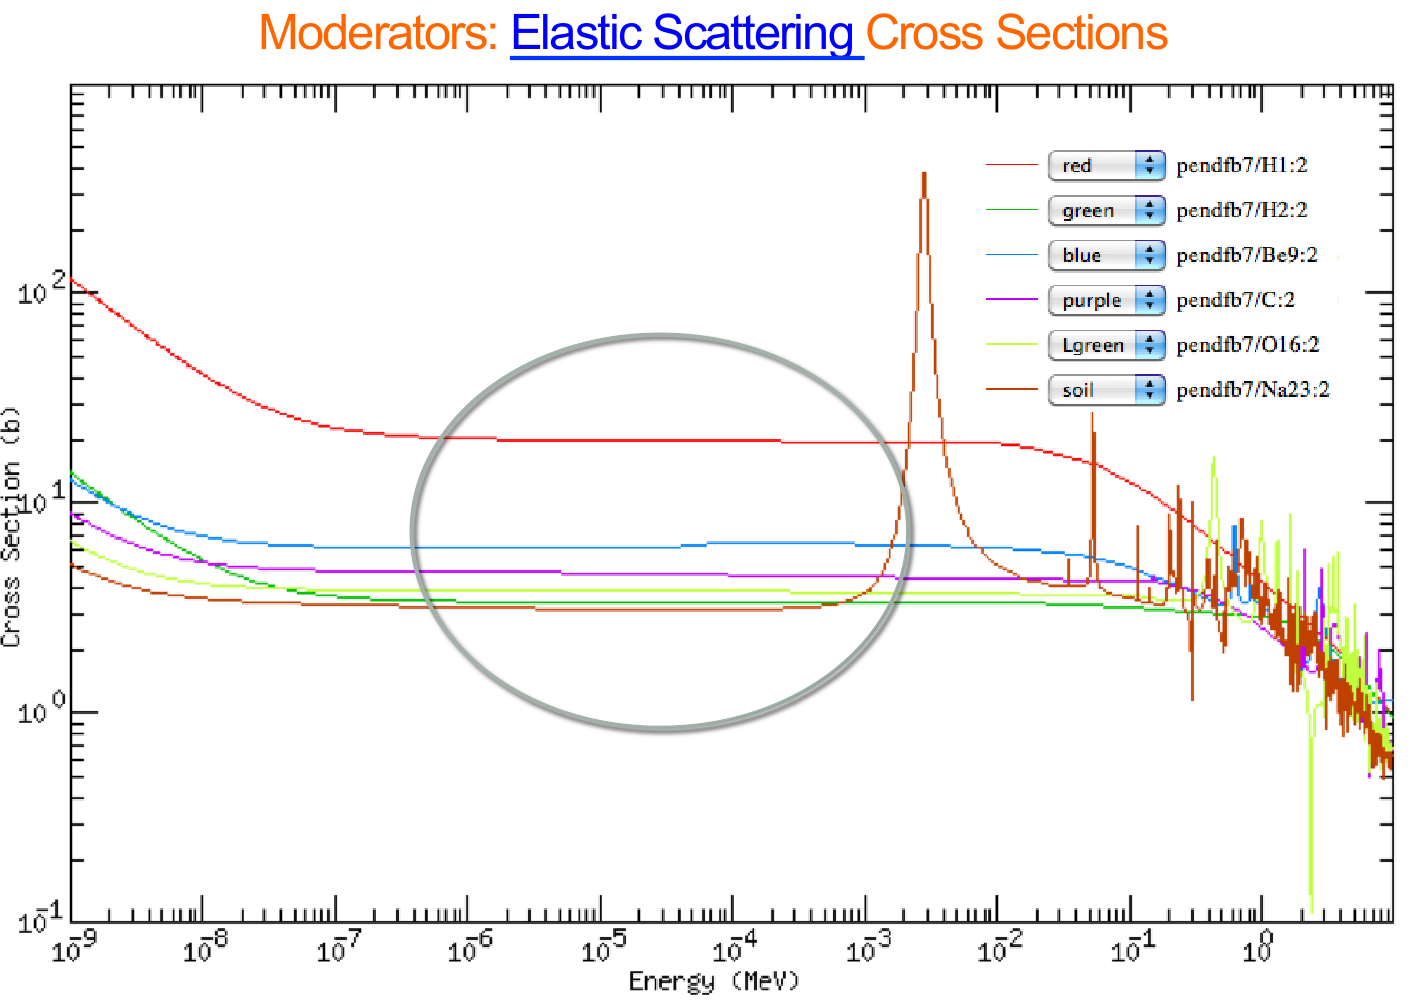
\includegraphics[width=4in]{images/scatter-xs-moderator.png}
  \\
  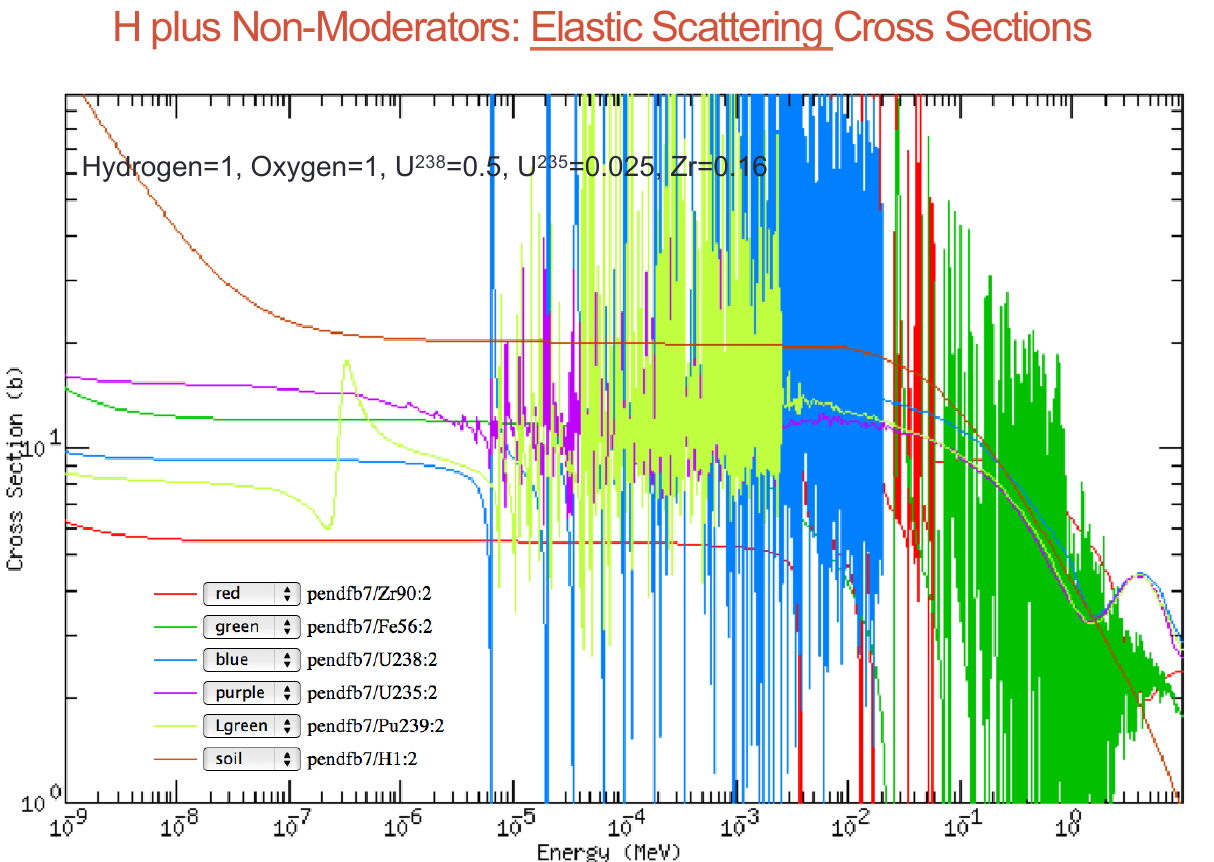
\includegraphics[width=4in]{images/scatter-xs-LWR.png}
  \caption{Elastic Scattering Cross Sections} \label{scatter-xs}
\end{figure}

\item Capture cross section as in Figure~\ref{capture-xs}: 
\begin{figure}
  \centering
  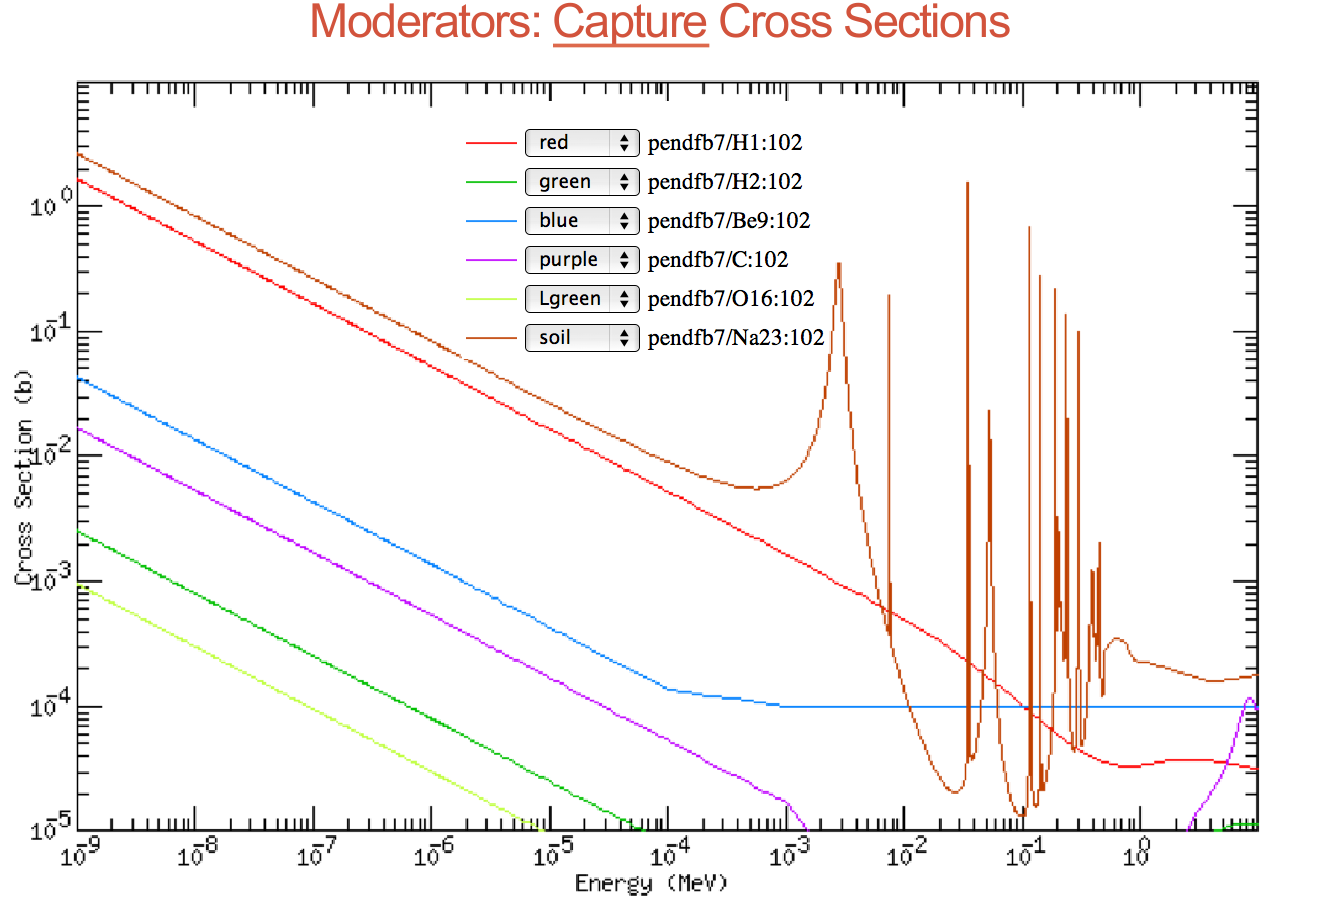
\includegraphics[width=4in]{images/capture-xs.png}
  \\
  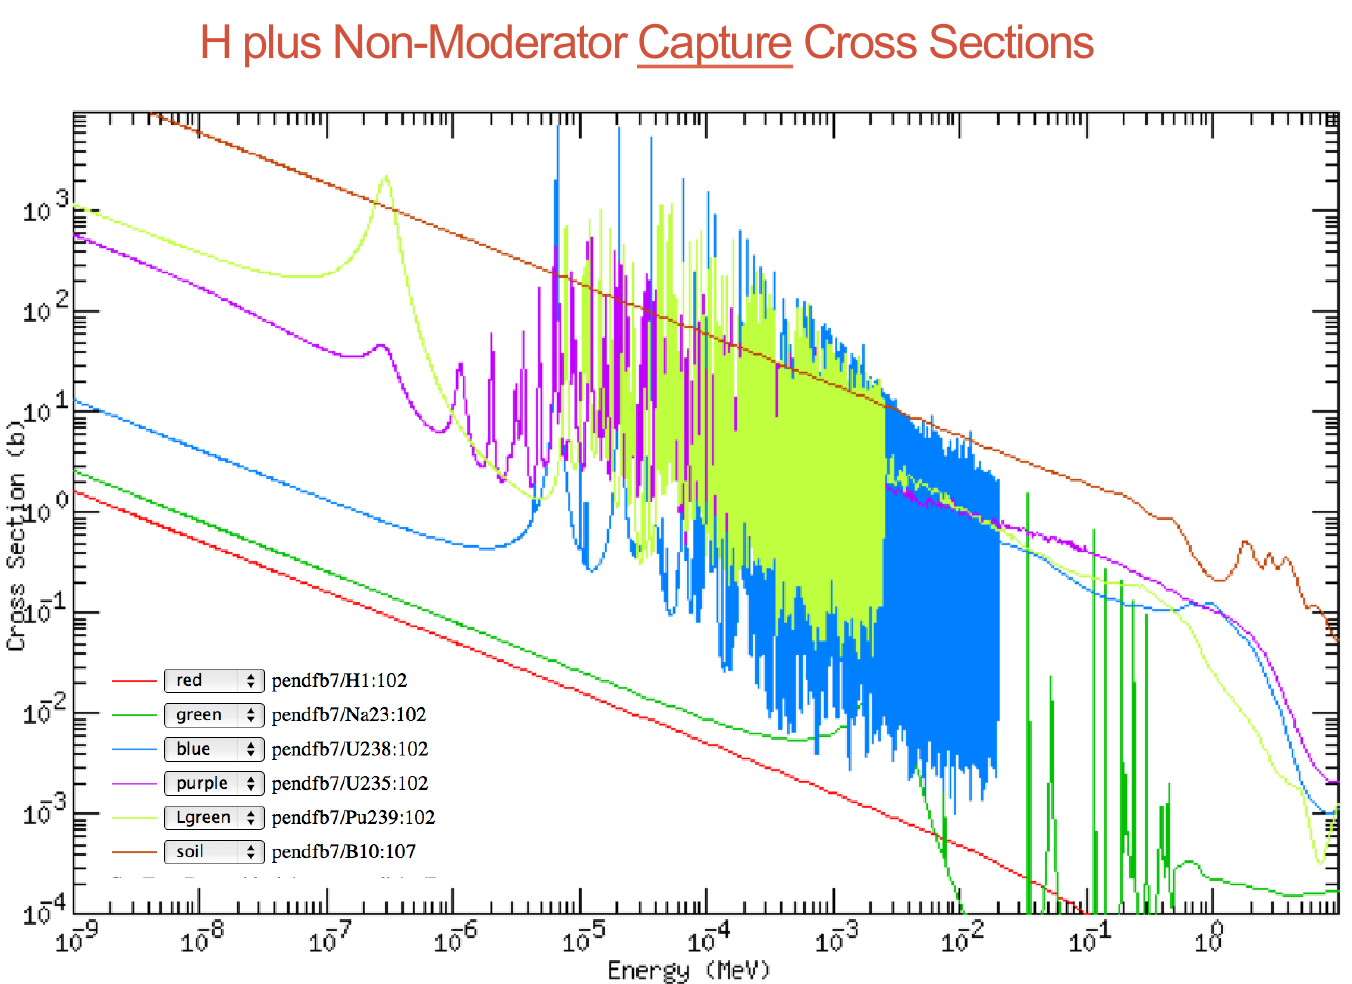
\includegraphics[width=4in]{images/capture-xs-2.png}
  \caption{Capture Cross Section} \label{capture-xs}
\end{figure}
\begin{enumerate}
\item H has no resonance; it has the highest scattering xs in LWR, so we can ignore any other isotopic's neutron scattering.   
\item Na has a huge resonance in 23 keV, and more resonances at higher energies because it is a heavy isotope.
\item Near zero energy,
\eqn{ \sigma(E\to 0) \propto \sqrt{\frac{kT}{AE}}    }
\item Resonance at 6 to 7 eV: U238. 
\item U235's thermal elastic xs is larger than 238's, and they both have resonance around the same range.   
\item A small resonance at .3 eV: Pu239 (its signiture is a super low energy scattering xs). 
\end{enumerate}

\item Given an unknown material type, all we care is to count the nucleus density of each material and look at it's xs. 
\item Average fission neutron energy: 2 MeV; average peak fission energy: 1 MeV; see fission sepctrum. 

\item Core decay heat after 1 day is about 1\% rated. 

\item Constants to know: 1u = 931.5 MeV. 
\end{enumerate}
%%%%%%%%%%%%%%%%%%%%%%%%% Qualify Exam End %%%%%%%%%%%%%%%%%%%%%%%%%%%%


\end{document}
